\section{Proposed software architecture}

\subsection{Overview}
The following chapter will go through: the chosen architecture patterns and design of the calendar system, the design patterns used to implement it and how the control flow of the program.
\newline
The figure below shows the class diagram of the proprosed system:

\begin{figure}[h]
\centering
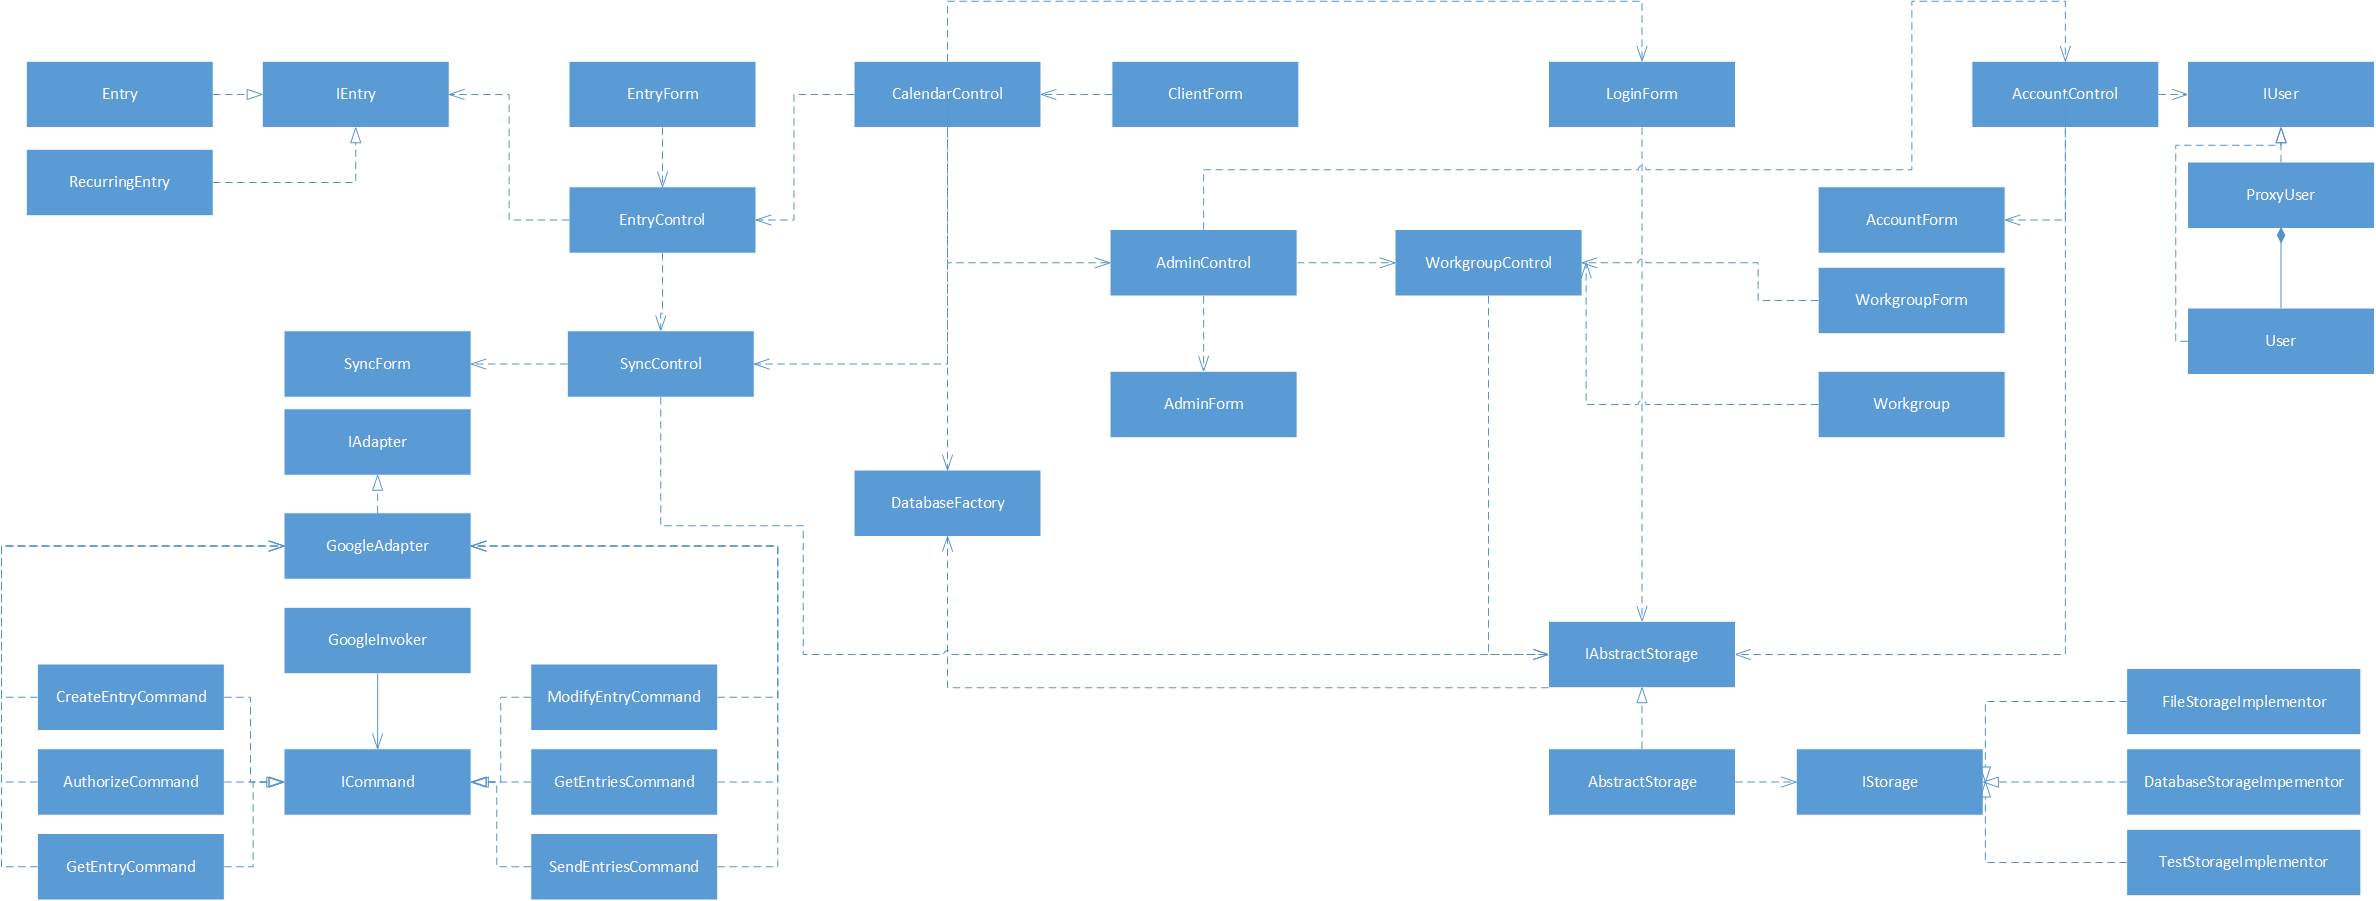
\includegraphics[scale = 0.3]{ClassDiagram}
\caption{Subsystems and their decomposition}
\end{figure}

\subsection{Subsystem decomposition}
The figure shows the subsystem decomposition of the User part of the program. The system is decomposed into subsystems which has logic handling one thing each, which means there’s a subsystem for entries, accounts, workgroups and sync. 
There’s a subsystem for handling the client (meaning the general UI) and directing the control flow. Then there’s a storage subsystem handling all interactions with the different storages (file and server storage). Finally there is the server subsystem holding the parts of the logic and model, handled by the server.
Control, model and view are still separated, but the logic has been split across multiple subsystems each handling something different.

\begin{figure}[h]
\centering
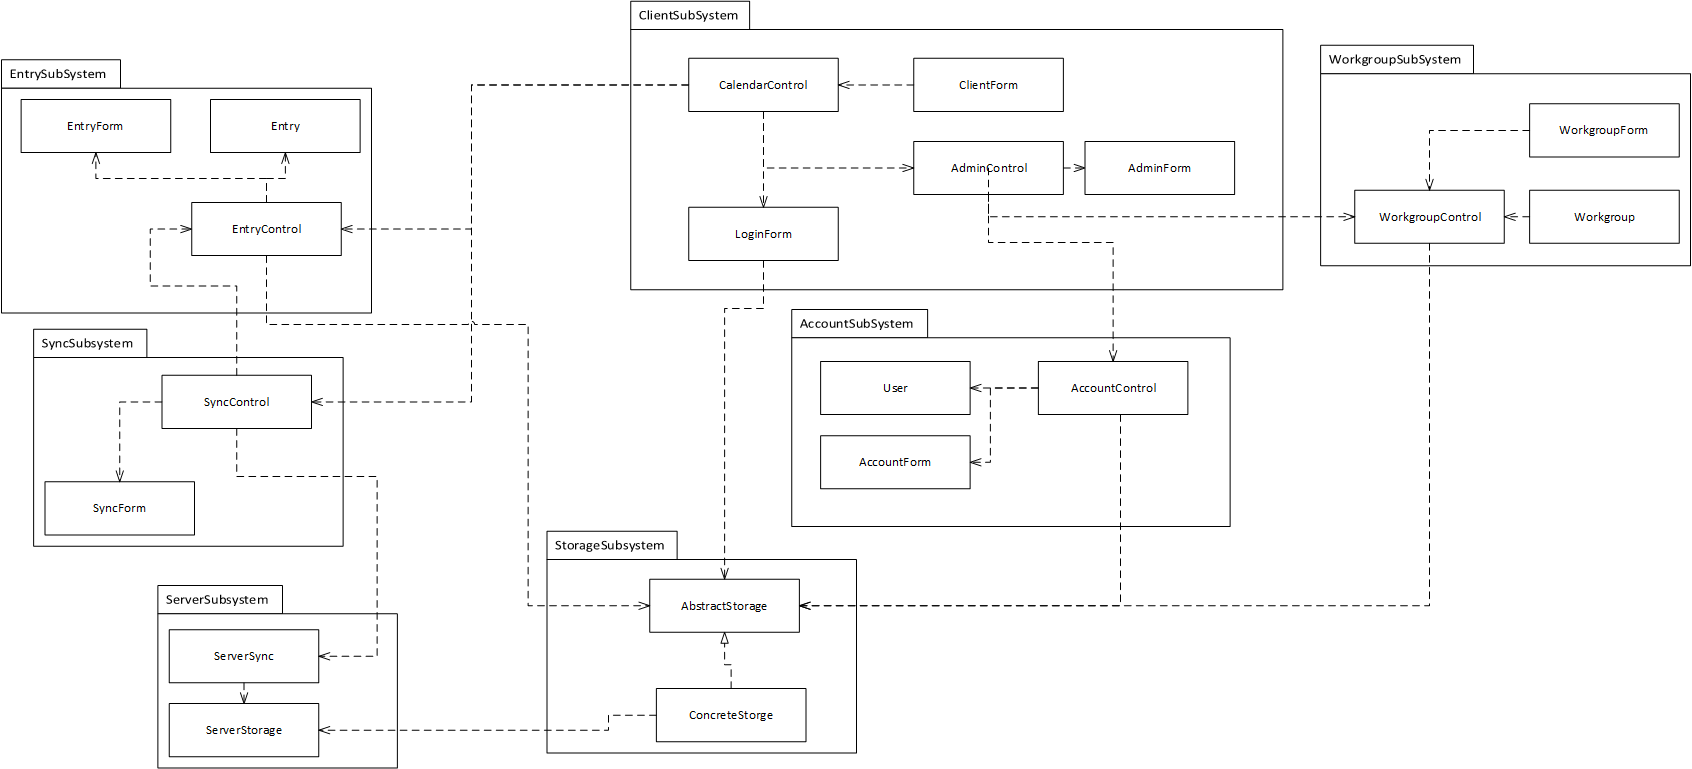
\includegraphics[scale = 0.35]{Subsystem}
\caption{Subsystems and their decomposition}
\end{figure}

\pagebreak

\subsection{Hardware/software mapping}
The figure shows the mapping of subsystems to hardware. All of the subsystems except ServerSubsystem are part of the client part of the system, meaning it runs on the computer a User is using. 
The StorageSubsystem runs on the client, communicating with the ServerSubsystem and in cases when the client is offline, uses the local cashed version of the calendar. The ServerSubsystem runs on the centralised server, allowing all clients to use it’s functionality.

\begin{figure}[h]
\centering
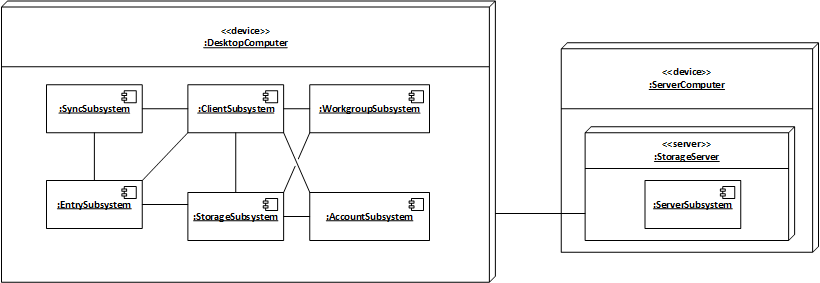
\includegraphics[scale = 0.7]{deployment}
\caption{Hardware/software mapping}
\end{figure}

\subsection{Persistent data management}
\flushleft{\textbf{Identifying persistent objects}}

The calendar system works with four entities, which need to be stored: The administrator and user entities, which need to be persistent, so accounts  doesn’t have to be made every time the system starts again. The workgroups also have to be saved since they would be useless unless persistent.
	Since it’s a calendar, the entries also need to be persistent, else it wouldn’t be a calendar, which is used to write down and remember events.
\flushleft{\textbf{Selecting a storage strategy}}

A mixed strategy has been chosen for the system, between relational database and flat file. The relational database will save all persistent information, which is then available online, while the flat file will save all relevant information to the specific user locally.
	This makes the system able to function off- and online. The relational database will be updated when online while also updating the local file. 
\newline
The figure below shows a RDBMS of our entities and their relation, showing how a database should store the data.

\begin{figure}[h]
\centering
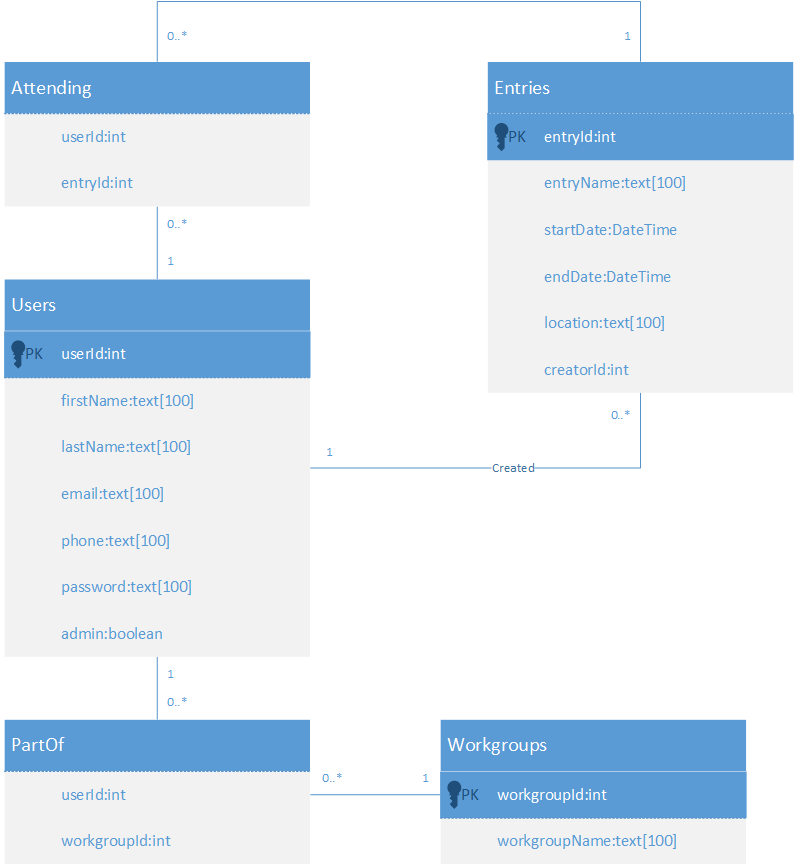
\includegraphics[scale = 0.6]{rdbms}
\caption{OO to RDBMS mapping}
\end{figure}

\pagebreak

\subsection{Access control and security}
There are only two kinds of actors that will be using the Calendar System: User and Administrator. Below is the access matrix, which specifies which parts of the Calendar System the two different actors will have access to.

\begin{figure}[h]
\centering
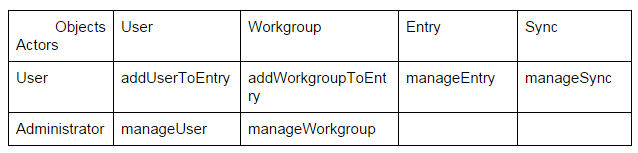
\includegraphics[scale = 0.8]{accessControl}
\caption{Access matrix for the Calendar System}
\end{figure}
The User is able to manage entries and manage which other calendars to sync their calendar with. A User is only able to add Users and Workgroup to an Entry, but is not able to change them.
The Administrator can manage Users and Workgroups, but doesn’t have anything to do with Entries and Sync.
The Server syncs a Users calendar with another calendar server, and as a part of that it is able to manage Entries.

\subsection{Global software control}
The server should be using threads as to allow multiple clients connected, updating their calendar at the same time. While the local client should be event-based, since it’s simpler than threads and there is no reason for the clients to use threads.

The figure below shows the subsystem decomposition with services:

\begin{figure}[h]
\centering
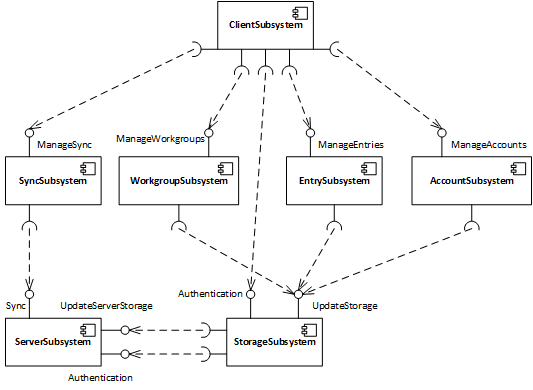
\includegraphics[scale = 0.7]{services}
\caption{Subsystem services}
\end{figure}

\subsection{Boundary conditions}
\flushleft{\textbf{Configuration use cases:}}

\begin{center}
    \begin{tabular}{ | l | p{10cm} |}
    \hline
    InstallClient & An administrator creates the calendar server, allowing the creation of new administrators and users, who can make use of the systems functions. \\ \hline
    \end{tabular}
\end{center}

\flushleft{\textbf{Start-up and shutdown use cases:}}
\begin{center}
    \begin{tabular}{ | l | p{10cm} |}
    \hline
    StartCalendarServer & An administrators starts the calendar server. As soon as the server is up and running, users will be able to synchronize their local calendar with the servers. \\ \hline
    \end{tabular}
\end{center}

\begin{center}
    \begin{tabular}{ | l | p{10cm} |}
    \hline
    ShutDownCalendarServer & An administrator stops the calendar server. Any changes made to entries, by users will instead be saved in the local storage and uploaded when the server becomes available again. \\ \hline
    \end{tabular}
\end{center}

\flushleft{\textbf{Exception use cases:}}

The calendar system can experience two major classes of system failures
\begin{itemize}
\item A network failure between the client and the server.
\item A failure causing the calendar server to unexpectedly terminate.
\end{itemize}
